\documentclass[12pt]{article}

\usepackage[utf8]{inputenc}
\usepackage[english]{babel}
\usepackage{amssymb}
\usepackage{amsfonts}
\usepackage{setspace}
\usepackage{algorithm}
\usepackage[noend]{algpseudocode}
\usepackage{amsmath}
\usepackage{graphicx}
\usepackage[margin=1in]{geometry}
\usepackage[hidelinks]{hyperref}
\usepackage{float}
\usepackage[danish]{varioref}
\usepackage{multirow}
\usepackage{hhline}
\usepackage{inconsolata}
\usepackage{etoolbox}
\usepackage[usenames,dvipsnames]{xcolor}
\usepackage{tikz}
\usetikzlibrary{positioning,shapes, shadows, arrows}
\usepackage{listings}

%%%%%%%%%%%%%%%%%%%%%%%%%
%        Theorem        %

\usepackage{amsthm}
\theoremstyle{definition}

\newtheorem{mydef}{Definition}

%                       %
%%%%%%%%%%%%%%%%%%%%%%%%%

%%%%%%%%%%%%%%%%%%%%%%%%%
%   subsubsubsection    %

\usepackage{titlesec}
\titleclass{\subsubsubsection}{straight}[\subsection]

\newcounter{subsubsubsection}[subsubsection]
\renewcommand\thesubsubsubsection{\thesubsubsection.\arabic{subsubsubsection}}

\titleformat{\subsubsubsection}
  {\normalfont\normalsize\bfseries}{\thesubsubsubsection}{1em}{}
\titlespacing*{\subsubsubsection}
{0pt}{3.25ex plus 1ex minus .2ex}{1.5ex plus .2ex}

\makeatletter
\def\toclevel@subsubsubsection{4}
\def\l@subsubsubsection{\@dottedtocline{4}{7em}{4em}}
\makeatother

\setcounter{secnumdepth}{4}
\setcounter{tocdepth}{4}

%                       %
%%%%%%%%%%%%%%%%%%%%%%%%%

%%%%%%%%%%%%%%%%%%%%%%%%%
%          Tikz         %

\tikzset{
  treenode/.style = {align=center, inner sep=0pt, text centered,
    font=\sffamily},
  arn_n/.style = {treenode, circle, black, font=\sffamily\bfseries, draw=white, fill=white, text width=1.5em}
}

%                       %
%%%%%%%%%%%%%%%%%%%%%%%%%

%%%%%%%%%%%%%%%%%%%%%%%%%
%       Algorithm       %

\usepackage{xspace}
\newcommand*\Let[2]{\State #1 $\gets$ #2}
\newcommand*\Returns[1]{\State \Return #1}
\newcommand*\Append[2]{\State $#1 << #2$}
\algrenewcommand\algorithmicrequire{\textbf{Input:}}
\algrenewcommand\algorithmicensure{\textbf{Output:}}
\renewcommand{\algorithmicforall}{\textbf{foreach}}
\algnewcommand{\Or}{\textbf{or}\xspace}
\algnewcommand{\Not}{\textbf{not}\xspace}
\algnewcommand{\In}{\textbf{in}\xspace}

%                       %
%%%%%%%%%%%%%%%%%%%%%%%%%

\setlength\parindent{0pt}
\usepackage[parfill]{parskip}

\definecolor{dark-blue}{HTML}{000080}
\definecolor{dark-green}{HTML}{008000}
\definecolor{pale-purple}{HTML}{94558D}
\definecolor{dark-purple}{HTML}{0000AA}
\definecolor{regular-purple}{HTML}{660099}
\definecolor{magenta}{HTML}{B200B2}
\definecolor{light-gray}{HTML}{FAFAFA}
\definecolor{dark-gray}{HTML}{2D2D2D}
\definecolor{comment}{HTML}{808080}
\definecolor{digit}{HTML}{0000FF}

\newcommand*{\FormatDigit}[1]{\textcolor{digit}{#1}}

\lstset{
	language=Ruby,
	prebreak=\raisebox{0ex}[0ex][0ex]{\ensuremath{\color{red}\space\hookleftarrow}},
	basicstyle=\footnotesize\ttfamily,
	%
	literate=%
    	{0}{{\FormatDigit{0}}}{1}%
        {1}{{\FormatDigit{1}}}{1}%
        {2}{{\FormatDigit{2}}}{1}%
        {3}{{\FormatDigit{3}}}{1}%
        {4}{{\FormatDigit{4}}}{1}%
        {5}{{\FormatDigit{5}}}{1}%
        {6}{{\FormatDigit{6}}}{1}%
        {7}{{\FormatDigit{7}}}{1}%
        {8}{{\FormatDigit{8}}}{1}%
        {9}{{\FormatDigit{9}}}{1}%
        {.0}{{\FormatDigit{.0}}}{2}% Following is to ensure that only periods
        {.1}{{\FormatDigit{.1}}}{2}% followed by a digit are changed.
        {.2}{{\FormatDigit{.2}}}{2}%
        {.3}{{\FormatDigit{.3}}}{2}%
        {.4}{{\FormatDigit{.4}}}{2}%
        {.5}{{\FormatDigit{.5}}}{2}%
        {.6}{{\FormatDigit{.6}}}{2}%
        {.7}{{\FormatDigit{.7}}}{2}%
        {.8}{{\FormatDigit{.8}}}{2}%
        {.9}{{\FormatDigit{.9}}}{2}%
        %{,}{{\FormatDigit{,}}{1}% depends if you want the "," in color
        {\ }{{ }}{1}% handle the space
		{æ}{{\ae}}1
        {ø}{{\o}}1
        {å}{{\aa}}1
        {Æ}{{\AE}}1	
        {Ø}{{\O}}1
        {Å}{{\AA}}1
        {~}{{$\scriptstyle{\sim}$}}1, % handle tilde ~
	%
	%emph={@param,@return},
	otherkeywords={},
	keywords=[2]{self},
	keywords=[3]{__init__},
	keywords=[4]{object},
	keywords=[5]{encoding, flags},
	keywords=[6]{map},
	%
	keywordstyle=\bfseries\color{dark-blue},
	keywordstyle={[2]\color{pale-purple}},
	keywordstyle={[3]\color{magenta}},
	keywordstyle={[4]\color{dark-blue}},
	keywordstyle={[5]\color{regular-purple}},
	keywordstyle={[6]\color{dark-purple}},
	keywordstyle={[7]\bfseries\color{black}},
    commentstyle=\itshape\color{comment},
    identifierstyle=\color{black},
	stringstyle=\bfseries\color{dark-green},
	%emphstyle=\bfseries,
	%
	numbers=left, % where to put the line-numbers
	numberstyle=\ttfamily\color{dark-gray},
	numbersep=5pt, % how far the line-numbers are from the code
	stepnumber=1,
	showstringspaces=false,
	backgroundcolor=\color{light-gray},
	tabsize=4,
	captionpos=b, % sets the caption-position to bottom
	breaklines=true % sets automatic line breaking
}

\linespread{1.3}

\begin{document}

\begin{titlepage}
    \vspace*{\fill}
    \begin{center}
      {\Huge Midtvejsrapport Bachelorproject}\\[0.7cm]
      {\Large Regular Expression Matching In Genomic Data}\\[0.4cm]
      {\large Rasmus Haarslev - nkh877}\\
      {\large Troels Thomsen - qvw203}\\[0.4cm]
      {\textbf{Supervisors:}\\
      Rasmus Fonseca\\
      Niels Bjørn Bugge Grathwohl\\
      Ulrik Rasmussen\\
      Martin Asser Hansen}\\
      {\small \textbf{April 30th 2015}}\\[0.3cm] 
      {\small Department of Computer Science}\\
      {\small University of Copenhagen}
    \end{center}
    \vspace*{\fill}
\end{titlepage}	

\clearpage
\pagenumbering{gobble}
\thispagestyle{empty}

\newpage

\tableofcontents
\newpage

\pagenumbering{arabic}

\section{Introduction}
\subsection{Motivation}

Institute for microbiology at University of Copenhagen has a large collection of sequenced DNA material stored on their servers. They estimate somewhere between two and three petabytes of data stored in FASTA and FASTQ files \textbf{NEED REF}.

Parsing and analysing this large amount of data poses several challenges. Searching through the files with simple text search is not advanced enough. DNA contains a lot of redundancy and variation over similar concepts, which means that two seemingly different sequences can have very similar functionality or interact with other components in a similar way. \\
This requires the search functionality to be able to allow for a great deal of variance and flexibility in the sequences which are searched for.

Currently, the state-of-the-art method for searching through genomic data is the scan-for-matches program, which, while performing very well, is not very user friendly \textbf{NEED REF} and have some unfortunate limitations when running many consecutive scans. However, scan-for-matches has easy-to-write pattern syntax compared REs, as well as the addition new syntax, which would make the equivalent REs extremely tedious to write.

Recently, the KMC group have developed a regular expression implementation called KMC, which so far has shown surprisingly competitive performance, compared to current industry standard engines\cite{two-pass-greedy}.

Since scan-for-matches outperforms the quite fast NR-grep (nondeterministic reverse grep), which is a pattern matching tool, created by the "search in page" facility at the University of Chile\cite{nrgrep}, we are hoping that optimized regular expressions running on the KMC engine will be able to outperform NR-grep and subsequently scan-for-matches.
If we could achieve a performance improvement over scan-for-matches, it would greatly benefit the microbiology team. As such we see this as a chance to make a unique contribution to ongoing and future research projects, while at the same time providing a chance for the KMC group to have their engine tested in a new scenario.

As such, we seek to solve the problem of translating the easy-to-write scan-for-matches patterns into the better-performing REs.


\subsection{Thesis Statement (TO BE REWRITTEN)}

We wish to determine the possibility of converting sequence analysis patterns used for scan-for-matches\cite{scan-for-matches}, into regular expressions\cite{crash-course-regex} and test their efficiency against the KMC\cite{kmc-website} engine.

Specifically we wish to solve the following problems:

\begin{itemize}
	\item Is it possible to programatically convert patterns used by the scan-for-matches program into regular expressions for the KMC engine? If not all patterns used by scan-for-matches then which ones?
	\item Is it possible to achieve speeds matching or exceeding scan-for-matches with the generated regular expressions and the KMC engine?
	\item Can we find weak extensions to regular expressions, which would enable us to support more or all scan-for-matches patterns?
\end{itemize}

\subsection{DNA/RNA}

Deoxyribonucleic acid (DNA) is a molecule, that is found in every known living organism, as well as many viruses. DNA encodes the genetic instructions, that the organism uses in the development and functioning of itself. DNA is a nucleic acid, which is one of three major macromolecules, that is essential for all known forms of life.

DNA can generally be described as an alphabet of 4 letters, which represent 4 different nucleobases, adenin (A), thymin (T), cytosin (C), and guanin (G) (figure \ref{dnabases}).

\begin{figure}[H]
\label{dnabases}
\begin{center}
	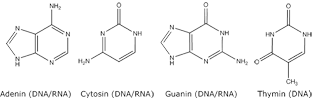
\includegraphics[scale=4]{dnabaserne.png}
\end{center}
\caption{The four different nucleobases found in the DNA nucleotides.\cite{DNA-biotechacademy}}
\end{figure}

\begin{mydef}
The alphabet, that makes up DNA sequences, denoted by $\mathcal{A}_{DNA}$ is:
\begin{center}
$\mathcal{A}_{DNA}$ = \texttt{\{ATCG\}}
\end{center}
\end{mydef}

The order of these nucleobases is what decides what function is encoded in any specific strand of DNA. A sequence of these nucleobases (a DNA sequence) is a sort of a genetic blueprint for proteins. During the production of proteins, a DNA sequence is either copied, or transcribed into ribonucleic acid (RNA), which decides which amino acids will be put together, which creates a corresponding protein.

Besides the 4 basic nucleobases, RNA uses uracil (U) instead of thymin, but they can be considered synonymous, and 11 ambiguity characters also exist.\cite{DNA-sciencedaily} These ambiguity characters were designed for positional variations in families of related genes. The ambiguity characters are named so because they represent  an uncertainty of which nucleobases is actually at that spot.

\begin{mydef}
The extended alphabet, that makes up DNA and RNA sequences, denoted by $\mathcal{A}_{ext}$ is:
\begin{center}
$\mathcal{A}_{ext}$ = \texttt{\{ATUGCYRSWKMBDHVN\}}
\end{center}
\end{mydef}

A DNA strand can bond with another DNA strand, containing the complementary nucleobases.

\begin{mydef}
\textbf{complementarity} is defined as a nucleobase capable of bonding with another nucleobase.
\end{mydef}

\begin{figure}[H]
	\label{Complementarity}
	\begin{center}
		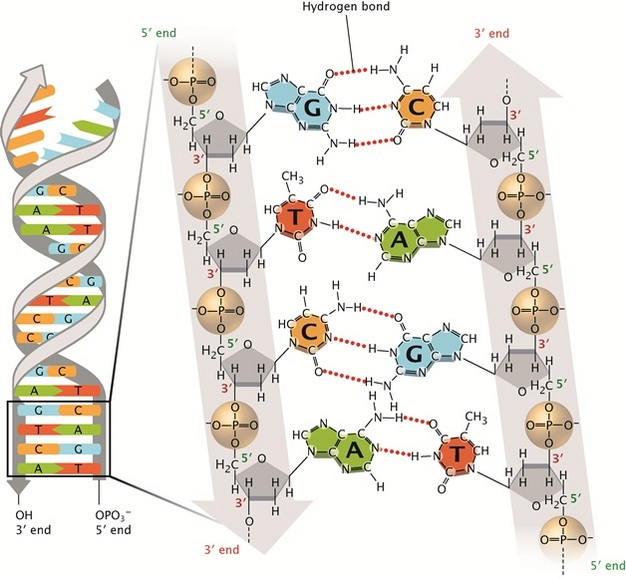
\includegraphics[scale=2.5]{complementarity.jpg}	
	\end{center}
	\caption{The four base pairs of complementarity.\cite{DNA-nature}}
\end{figure}

Sometimes, you may wish to express a DNA sequence's complementary DNA sequence. This is called the reverse complement of a given DNA sequence.

\begin{mydef}
A DNA sequence containing the complementary bases of another DNA sequence, is called the \textbf{reverse complement} of the latter sequence.
\end{mydef}

\subsection{What is scan-for-matches?}

Scan for matches is a program developed by Ross Overbeek, David Joerg and Morgan Price\cite{scan-for-matches}, which is able to locate complex DNA patterns, such as looking for a random 8 character sequence, repeated 20 characters ahead, and in reverse. These patterns will be referred to as \textit{patscan patterns}, while the program itself will be referred to as \textit{scan-for-matches}.

The patscan language can be broken down into a few simple components or tokens, which we will refer to as sub-patterns. We have divided the sub-patterns into the following classes:

\begin{mydef}
The sub-patterns, that consists only of a consecutive sequence of characters from $\mathcal{A}_{ext}$, is denoted as a \textbf{sequence} (Example: \texttt{AGTCT})
\end{mydef}

\begin{mydef}
The sub-patterns, that consists of a consecutive sequence of characters from $\mathcal{A}_{ext}$, followed by square brackets, containing three numbers (each representing \textbf{mismatches}, \textbf{insertions}, and \textbf{deletions} respectively), is denoted as a \textbf{combination} (Example: \texttt{AGTCT[1,0,0]})
\end{mydef}

\begin{mydef}
The sub-patterns, that consists of a number, $a \geq 0$, followed by exactly three dots, followed by a number, $b \geq a$, is denoted as a \textbf{range} (Example: \texttt{2...4})
\end{mydef}

\begin{mydef}
The sub-patterns, that consists of a string, denoted as a \textbf{variable name}, followed by an equal sign, and then a \textbf{sequence}, is denoted as a \textbf{variable assignment} (Example: \texttt{p1=AGTCT})
\end{mydef}

\begin{mydef}
The sub-patterns, that consists only of a \textbf{variable name}, is denoted as a \textbf{variable usage} (Example: \texttt{p1})
\end{mydef}

The complete grammar we use for our translation can be found in section \ref{Patscan grammar}.

The most notable of the patscan format's features, is the possibility to search for mismatches, insertions and deletions in a given sequence or stored sequence. The sequence \texttt{AGTCT} can be extended to \texttt{AGTCT[1,1,1]} in order to match up to one mismatch, up to one insertion, up to one deletion or any combination thereof. \\
This means that a sequence of length $n$ with a single mismatch will yield $n^1+1$ possible matches. \texttt{AGTCT[1,0,0]} will for instance match any of the following, where \_ represents a mismatch.

\texttt{AGTCT, \_GTCT, A\_TCT, AG\_CT, AGT\_T, AGTC\_}

If we extrapolate into $m$ mismatches, $d$ deletions, and $i$ insertions, we quickly find ourselves with approximately $n^{m^{d^{i}}}+1$ possible matches since all of our mismatches can be combined with all of our deletions, which in turn can be combined with all of our insertions. This is not something easily replicated with regular expressions, as we shall see in the following sections.

Another powerful feature of patscan is the ability to store a sub-pattern match in a named variable. If a match is found for the named variable in the beginning of a pattern for instance, this match can then be referenced later in the same pattern, by using the variable name. \\
An example of this could be the pattern \texttt{p1=2...4 10...20 \~{}p1}. This pattern will match the contents of \texttt{p1}, followed by any 10 to 20 characters, followed by the match stored in \texttt{p1}, but with the reverse complement as denoted by the \texttt{\~{}}.\\
This is similar to the back-referencing functionality for capturing groups, which many popular regular expression implementations support.%\cite{indsæt citation her.}

Combining this combination notation with the ability to store sequences in variables and matching them further down the pattern, makes the patscan language very compact compared to regular expressions. \\
A pattern as simple as \texttt{p1=8...16 10...50 ~p1[2,0,1]} describes a complex relationship, which cannot easily be discovered through REs.

We will try to translate patscan patterns into regular expressions, and run them on the KMC group's RE engine. We hope to achieve similar, or better speeds to those of scan-for-matches, while also achieving the same search results.

\subsection{Regular Expressions (TODO)}

In order to talk about regular expressions, we need to be able to talk in general terms of languages. We can define a language as a subset of the infinite set of words or symbols, chosen from a finite alphabet. An alphabet with the letters $\{\alpha, \beta\}$ might for an example form the words $\alpha\beta$, $\beta\alpha$, $\alpha\alpha\beta$ or any such conbination of any length, thus forming an infinite set of words.\\

\begin{mydef} Given an alphabet $\Sigma$ consisting of a finite set of characters, we can define a regular expression $E$.
	\begin{enumerate}
		\item An expression containing a single letter $\alpha$ from our alphabet $\Sigma$: $E = \alpha$
		
		\item A combination of the two regular expressions $E_1$ and $E_2$:
		\begin{eqnarray}
			E &=& E_1 | E_2 \\
			E &=& E_1E_2 \\
			E &=& E_1^* \\
		\end{eqnarray}
	\end{enumerate}	
\end{mydef} 

We can also interpret the regular expression $E$ from the alphabet $\Sigma$, as a language denoted by $\mathcal{L}(E)$. \\

\begin{mydef} The language $\mathcal{L}(E)$ for the regular expression $E$ from the alphabet $\Sigma$, can be defined as.

	\begin{enumerate}
		\item For single-letter expressions we have
			\begin{eqnarray}
				\mathcal{L}(0) &=& \emptyset \\
				\mathcal{L}(\alpha) &=& \{\alpha\}
			\end{eqnarray}
			Where $\alpha \in \Sigma$
			
		\item For combined expressions we have
			\begin{eqnarray}
				\mathcal{L}(E_1|E_2) &=& \mathcal{L}(E_1) \cup \mathcal{L}(E_2) \\
				\mathcal{L}(E_1E_2) &=& \mathcal{L}(E_1) \odot \mathcal{L}(E_2) \\
				\mathcal{L}(E^*) &=& \bigcup^{\infty}_{n = 0}\mathcal{L}(E^n)
			\end{eqnarray}
			Where $\mathcal{L}(E_1) \odot \mathcal{L}(E_2) = \{w_1w_2 \ |\  w_1 \in \mathcal{L}(E_1), w_2 \in \mathcal{L}(E_2)\}$, and where $E^n$ denotes E combined with itself $n$ times.
	\end{enumerate}
\end{mydef}

\newpage

\section{Methods}
\subsection{PatScan as regular expressions (TO BE WRITTEN)}

\subsubsection{Grammar (TO BE WRITTEN)}
\label{Patscan grammar}

We have defined the following grammar for the patscan language:

\begin{figure}[H]
\begin{tabular}{|lcll|}
	\hline
	$Prog$ & $\rightarrow$ & $StmtSeq$ & \\
	$StmtSeq$ & $\rightarrow$ & $Stmt\ StmtSeq$ & \\
	$StmtSeq$ & $\rightarrow$ & $Stmt$ & \\
	$Stmt$ & $\rightarrow$ & $Exp$ & \\
	$Stmt$ & $\rightarrow$ & $LVal\ =\ Exp$ &  \textcolor{red}{Variable assignment} \\
	$Stmt$ & $\rightarrow$ & $LVal$ & \textcolor{red}{Variable usage} \\
	$LVal$ & $\rightarrow$ & Id $Combi$ & \\
	$LVal$ & $\rightarrow$ & {\raise.17ex\hbox{$\scriptstyle\mathtt{\sim}$}} Id $Combi$ & \\
	$Exp$ & $\rightarrow$ & \textbf{num} ... \textbf{num} & \textcolor{red}{Range} \\
	$Exp$ & $\rightarrow$ & $Seq\ Combi$ & \\
	$Seq$ & $\rightarrow$ & \textbf{char} $Seq$ & \\
	$Seq$ & $\rightarrow$ & \textbf{char} & \\
	$Combi$ & $\rightarrow$ & [\textbf{num},\textbf{num},\textbf{num}] & \\
	$Combi$ & $\rightarrow$ & $\epsilon$ & \\
	\hline
\end{tabular}
\caption{PatScan grammar}
\end{figure}

\subsubsection{Mismatches, Insertions and Deletions (TO BE RESTRUCTURED)}

Combination sub-patterns can have the following form, which allows for mismatches, insertions and deletions in the sub-pattern. 
\begin{equation}
	Sequence[m, i, d] \ \ \{m, i, d \in \mathbb{N}_0 \}
\end{equation} 

This notation allows for up the given number of mismatches, insertions or deletions. This means we for example can have $m$ mismatches and $i$ insertions, but not necessarily $d$ deletions.

This kind of notation does not exist in REs. One way to represent these sub-patterns as REs is by constructing every possible combination of the sequence, matching the patscan notation.

Starting with mismatches only, writing a general algorithm to translate this example is fairly simple, but becomes increasingly difficult, as the sequence becomes longer, and the number of allowed mismatches increases.

We tried the following approaches to solving this problem, but ultimately decided on a divide and conquer algorithm. 

\subsubsubsection{Recursion (TO BE REWRITTEN)}

Solving the problem with recursion one might take each character one at a time, and look at all the possibilities for that character.

This way we could construct a recursion tree containing all possible combinations, no matter how many mismatches are allowed.

For mismatches the recursion tree would add two new branches per iteration. The first iteration of \texttt{AGCTC[2,0,0]} would add the branches

\begin{eqnarray}
	Left\ branch &=& A\{GCTC[2,0,0]\} \\
	right\ branch &=&\ \hat{}A\{GCTC[1,0,0]\}
\end{eqnarray}

The left branch will continue recursively with \texttt{GCTC[2,0,0]}, and the right branch will do the same but with only one mismatch available, since we already chose $A$ as our first mismatch. Thus we must choose all possibilities from $N \in \{n, \hat{}n\}$ as a new branch, every time we take a recursion step.
On our leafs we will have a string with a unique combination of mismatches.

Adding deletions and insertions will increase the size of $N$, thus drastically increasing the recursion depth. The recursion does not stop until every combination is found. This means that if the sequence is large enough (This can happen already at a length of 20, if not earlier, depending on the number of mismatches, insertions, and deletions), the program will reach maximum recursion depth or run out of memory before completing.

\subsubsubsection{Divide and Conquer}

To solve the recursion depth problem, we thought of using a divide and conquer algorithm instead, which would reduce the recursion depth to $log(n)$. This works by splitting the sequence in two halves per recursion, such that at the deepest recursion level, we have a single sequence of only a single character. 

\begin{figure}[H]
\begin{tikzpicture}[->,>=stealth',level/.style={sibling distance = 5cm/#1,
  level distance = 1.5cm}] 
\node [arn_n] {abcd}
	child{ node [arn_n] {ab} 
		child{ node [arn_n] {a}}
		child{ node [arn_n] {b}}                            
	}
    child{ node [arn_n] {cd}
		child{ node [arn_n] {c}}
		child{ node [arn_n] {d}}
	}
; 
\end{tikzpicture}
	\centering
	\caption{Tree structure, showing the steps taken by the algorithm during the divide step.}
	\label{fig:tree_example}
\end{figure}

After dividing the sequence into characters, we have to conquer each sub-problem. On the lowest recursion level (where the sequence is a single character), the algorithm will return a list of all possibilities, which that character can be.

For character 'a' from figure \ref{fig:tree_example}, we have the following possibilities for mismatches and deletions

\begin{center}
	{a, \^{}a, \_}
\end{center}

as well as the following for insertions

\begin{center}
	\texttt{.\{1\}a, .\{2\}a, $\cdots$, .\{n\}a} \\
	\texttt{a.\{1\}, a.\{2\}, $\cdots$, a.\{n\}}
\end{center}

A list of all these possibilities is then returned, and it can be combined with the list received from the 'b' recursion.

These lists are combined by combining each outcome from the first list, and combining it with each outcome of the second list. The total number of mismatches, insertions, and deletions are being kept track of, and if combining two outcomes will result in more mismatches, insertions, or deletions than the maximum allowed, then it is skipped.

\begin{spacing}{0.8}
\begin{algorithm}
	\caption{find\_combinations}
	\label{alg:find_combinations}
  	\begin{algorithmic}[1]
    		\Require
    			\Statex seq - sequence string to be translated
    			\Statex $m_{max}$ - allowed number of mismatches
    			\Statex $d_{max}$ - allowed number of deletions
    			\Statex $i_{max}$ - allowed number of insertions
    		\Ensure
    			\Statex List of all possible combinations
		\Statex
    		\If{$seq.length > 1$}
    			\Let{left\_tree}{self(seq[0..(seq.length/2).floor-1], $m_{max}$, $i_{max}$, $d_{max}$)}
    			\Let{right\_tree}{self(seq[(seq.length/2).floor..-1], $m_{max}$, $i_{max}$, $d_{max}$)}
    		\Else
    			\Returns{List of all mismatch, insertion, and deletion combinations of seq}
    		\EndIf
    		\State
    		\Let{combined}{empty list}
    		\Let{unique\_combinations}{empty hash table}
    		\ForAll{LL \In left\_tree} \Comment{LL: Left leaf}
    			\ForAll{RL \textbf{in} right\_tree} \Comment{RL: Right leaf}
    				\If{$LL.m + RL.m > m_{max}$ \Or $LL.d + RL.d > d_{max}$ \Or $LL.i + RL.i > i_{max}$}
    					\State continue
    				\EndIf
    				\If{\Not LL.seq + RL.seq \In unique\_combinations.keys}
    					\Append{unique\_combinations}{LL.seq + RL.seq}
    					\Append{combined}{LL + RL}
    				\EndIf
    			\EndFor
    		\EndFor
    		\Returns{combined}
  	\end{algorithmic}
\end{algorithm}
\end{spacing}

\newpage
\subsubsubsection{Redundancy}

With this implementation, we will have a lot of redundancy, when translating insertions. This comes from the fact, that we wish to construct all possible combinations, and that we do it recursively.

If we look at the combination sequence \texttt{ab[0,1,0]}, the possible outcomes of \texttt{a} (at the lowest level of recursion) can be \texttt{a}, \texttt{.a}, and \texttt{a.}, and the same for \texttt{b}. Combining these, we will have two different cases of \texttt{a.b} (\texttt{a. b} and \texttt{a .b}). It is redundant to keep both, and by keeping it, will create even more redundancy in the upper levels of the recursion.

On the first conquer step, we will have $r_0$ redundant cases, which is calculated using (4), where $i_{max}$ is the number of allowed insertions, and $n$ is the number of characters in the sequence.
\begin{eqnarray}
	r_0 = n\sum^{i_{max}}_{i=1} i
\end{eqnarray}

On the next level, we have $r_1$ redundant cases, calculated using (5), where $m=1$ if any number of mismatches are allowed, $i$ is the number of insertions allowed, and $d=1$ if any number of deletions are allowed.
\begin{eqnarray}
	r_1 \approx r_0(1 + m + 2i + d)
\end{eqnarray}

To calculate further redundancy, I will use $c = (1 + m + 2i + d)$, corresponding to the above. We can then calculate the total amount of redundancy, via induction:
\begin{eqnarray}
	r_n \approx r_{n-1}c_{n-1}^2
\end{eqnarray}

Here, $n$ is the recursion depth, and will thus go up to $logm$, where $m$ is the length of the patscan sequence.

This is only an approximation, as some combinations will be thrown away if there are more mismatches, insertions, or deletions than is allowed. Furthermore, the recursion depth varies in the recursion branches based on the length of the original string, like in figure \ref{fig:recursion_depth_example}.

\begin{figure}[H]
\begin{tikzpicture}[->,>=stealth',level/.style={sibling distance = 5cm/#1,
  level distance = 1.5cm}] 
\node [arn_n] {abc}
	child{ node [arn_n] {a}}
    child{ node [arn_n] {bc}
		child{ node [arn_n] {b}}
		child{ node [arn_n] {c}}
	}
; 
\end{tikzpicture}
	\centering
	\caption{Tree structure, how recursion depth varies in different branches.}
	\label{fig:recursion_depth_example}
\end{figure}

Despite of this inaccuracy, it is still trivial, that the amount of redundancy in larger patterns is extremely excessive, as it translates directly into additional runtime.

Avoiding this redundancy is very important, and relatively trivial. Every time two cases are combined, it is used as a key in a hash table, and its value set to true. The value doesn't matter, all that matters is that the hash table now has this combination as a key.

Every time we make a new combination, we check if that combination already exists, and if it does, we simply skip it.

We can look up in a hash table in $O(1)$ time, which doesn't increase the runtime by much. However, we will end up with a significantly lower runtime in the long run, as all redundancy is sorted out.

\subsubsection{Variable assignments \& usage}

Variable assignment is when you have a pattern of some sort, that you assign to a variable, so that it may be reused later. Any kind of non-variable pattern may be used in a variable pattern. Hence, we have three different variable assignments:

\texttt{p1=ATCG} \\
\texttt{p2=ATCG[2,0,0]} \\
\texttt{p3=2...4}

These assignments can be referenced by using the variable name. An example of such usage could be

\texttt{q1=ACCT 2...5 q1}

In addition just referencing the variable, a variable may also be inverted. This is denoted by using a tilde character prepended to the variable:

\texttt{{\raise.17ex\hbox{$\scriptstyle\mathtt{\sim}$}}q1}

Here, inversion refers to the reverse complement of the sequence stored in the variable.

Sequence and combination assignments are implemented by translating the sequence/combination and storing the translated regular expression in a table, with the variable name as the key. Then, if the variable is used later in the patscan pattern, the translated sequence/combination may be placed into the full regular expression. This way, there are no actual referencing in the regular expression, which we want to keep regular.

Assignment of a range is something we have chosen not to implement, as it can't be implemented without the use of back-referencing. This is because there's no way of knowing what a range will actually be besides x-y random characters. Because of this inherent ability to change, depending on where in the file the engine is matching, it is not possible to 'hard code' it as a regular expression.

Using back-referencing in our implementation will cause our RE patterns to lose regularity, and with that, performance.

\subsection{Correctness (TO BE WRITTEN)}

\subsection{Runtime (TO BE WRITTEN)}

\subsection{Data Analysis (TO BE WRITTEN)}

\section{Results (TO BE WRITTEN)}

\subsection{Experiment design (TO BE WRITTEN)}

\subsection{Experiment results (TO BE WRITTEN)}

\section{Conclusion (TO BE WRITTEN)}

\newpage

\pagenumbering{gobble}
\bibliographystyle{plain}
\nocite{*}
\bibliography{litterature}

\end{document}
